In order to see the big picture, we decided to use an approach from Cadle \& Yeates\cite[ch.~8.3.1]{caye} known as a \emph{work breakdown structure}. The work breakdown structure is organized in a hierarchical tree structure, where each new level in the tree is created by dividing a task into subtasks, as shown in Figure \ref{fig:breakdown}.

\begin{figure}[hbtp]
    \centering
	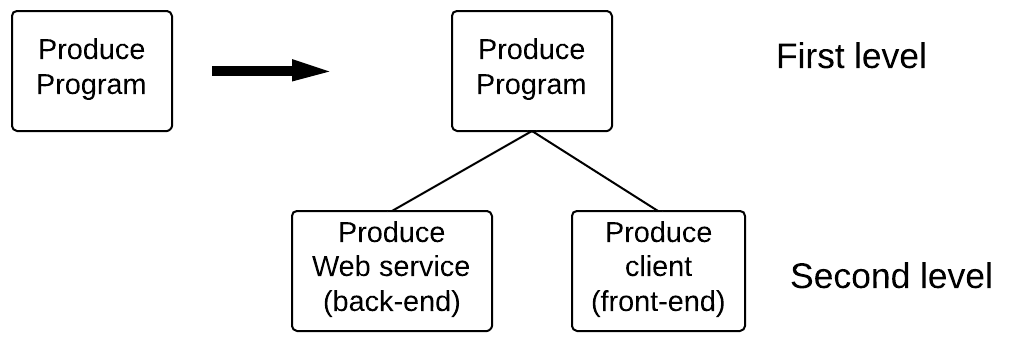
\includegraphics[scale=0.25]{./Empiri/Planning/img/wbslevels.png}
	\caption{Example work breakdown structure} \label{fig:breakdown}
\end{figure}

The division of tasks into smaller components is an iterative process, which stops when the resulting tasks are small enough to be considered a suitable assignment for one man or, more subjectively, when it simply does not make sense to divide it any further.

Using the above approach, we created the work breakdown structure found in Appendix \ref{app:workbreak}. Our work breakdown structure has four levels of depth, each one representing a different level of abstraction.